\iffalse
\documentclass[a4paper,12pt,twocolumn]{article}
\usepackage{graphicx}
\usepackage[margin=0.5in]{geometry}
\usepackage[cmex10]{amsmath}
\usepackage{array}
\usepackage{gensymb}
\usepackage{booktabs}
\title{Line Assignment}

\author{Ravi Sumanth Muppana- FWC22003}
\date{September 2022}
\providecommand{\norm}[1]{\left\lVert#1\right\rVert}
\providecommand{\abs}[1]{\left\vert#1\right\vert}
\let\vec\mathbf
\newcommand{\myvec}[1]{\ensuremath{\begin{pmatrix}#1\end{pmatrix}}}	
\newcommand{\mydet}[1]{\ensuremath{\begin{vmatrix}#1\end{vmatrix}}}
\providecommand{\brak}[1]{\ensuremath{\left((#1\right)}}
\begin{document}
\maketitle
\section{Problem:}
\fi
Show that if the diagonals of a quadrilateral bisect each other at right angles, then it is a rhombus.
\begin{figure}[!h]
	\centering
	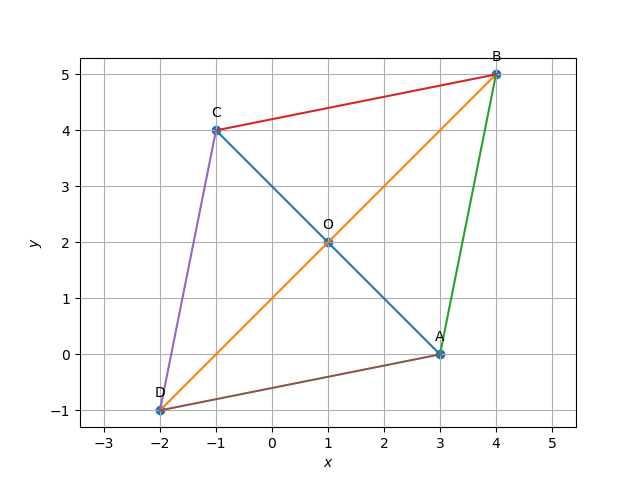
\includegraphics[width=\columnwidth]{chapters/9/8/1/3/figs/rhombus.png}
	\caption{Rhombus}
	\label{fig:9/8/1/3}
\end{figure}
\\
\solution See Fig. 
	\ref{fig:9/8/1/3}.
\iffalse
\maketitle
\section{Solution:}
\subsection{Theory:}
\fi
From the given information,
\begin{align}
	\label{eq:9/8/1/3-mid}
	\frac{\vec{B}+\vec{D}}{2}
	&=	
	\frac{\vec{A}+\vec{C}}{2}
	\\
	\brak{\vec{B}-\vec{D}}^{\top}&
	\brak{\vec{A}-\vec{C}} = 0
	\label{eq:9/8/1/3-orth}
\end{align}
From 
	\eqref{eq:9/8/1/3-mid},
\begin{align}
	\vec{B}-\vec{A}
	=	
	\vec{C}-\vec{D}
	\label{eq:9/8/1/3-pgm}
\end{align}
which, from  
	  \eqref{eq:two-pgm}, 
is the definition of  a parallelogram.
Further, substituting
\begin{align}
	\vec{B}-\vec{D} &= \brak{\vec{B}-\vec{A}} +  
	\brak{\vec{A}-\vec{D}}
	\\
	\vec{A}-\vec{C} &= \brak{\vec{A}-\vec{B}} +  
	\brak{\vec{B}-\vec{C}}
\end{align}
in 
	\eqref{eq:9/8/1/3-orth},  
\begin{multline}
	\sbrak{\brak{\vec{B}-\vec{A}} +  
	\brak{\vec{A}-\vec{D}}}^{\top}
	\sbrak{ \brak{\vec{A}-\vec{B}} +  
	\brak{\vec{B}-\vec{C}}} = 0
	\\
	\implies 
-\norm{\vec{B}-\vec{A}}^2 + \brak{\vec{B}-\vec{A}}^{\top}\brak{\vec{B}-\vec{C}} + 
\\
	\brak{\vec{A}-\vec{D}}^{\top}\brak{\vec{A}-\vec{B}} + 
\brak{\vec{A}-\vec{D}}^{\top}
\brak{\vec{B}-\vec{C}} = 0
	\label{eq:9/8/1/3-org}
\end{multline}
From
	\eqref{eq:9/8/1/3-pgm},
\begin{align}
	\vec{B}-\vec{C}
	=	
	\vec{A}-\vec{D}
	\\
	\implies \brak{\vec{B}-\vec{A}}^{\top}\brak{\vec{B}-\vec{C}} +
	 \brak{\vec{A}-\vec{D}}^{\top}\brak{\vec{A}-\vec{B}} =\vec{0}
	\label{eq:9/8/1/3-orth-pf}
\end{align}
and 
\begin{align}
\brak{\vec{A}-\vec{D}}^{\top}
\brak{\vec{B}-\vec{C}} = \norm{\vec{B}-\vec{C}}^2
	\label{eq:9/8/1/3-orth-eq}
\end{align}
Substituting from

	\eqref{eq:9/8/1/3-orth-pf}
and
	\eqref{eq:9/8/1/3-orth-eq}
in
	\eqref{eq:9/8/1/3-org},

\begin{align}
\norm{\vec{A}-\vec{B}}^{2}
= \norm{\vec{B}-\vec{C}}^2
\end{align}
which means that the adjacent sides of the parallelogram are equal. Thus, the quadrilateral is a rhombus
\iffalse


Since
Let us assume two vectors $\vec{C}-\vec{B}-\vec{A}$ and $\vec{C}-\vec{B}$ for sides $BA$ and $CB$. The diagonals $AC,BD$ are the addition and subtraction of the two vectors:
\begin{align}
	&\vec{(B-A)} = \vec{C}-\vec{B}-\vec{A}\\
	&\vec{(C-B)} = \vec{C}-\vec{B}\\
	&\vec{(C-A)} = \vec{(C-B)} +\vec{(B-A)}\\
	&\vec{(C-A)} = \vec{b+a}\\
	&\vec{(D-B)} = \vec{b-a}\\
\end{align}
%\subsection{Mathematical Calculation:}
Let the two diagonals be $\vec{a+b}$, $\vec{b-a}$. Since the diagonals are at right angle to each other,
\begin{align}
&0 = \vec{(a+b)^T}\vec{(b-a)}\\	
&||\vec{C}-\vec{B}||^2 - ||\vec{C}-\vec{B}-\vec{A}||^2 = 0\\
&||\vec{C}-\vec{B}|| = ||\vec{C}-\vec{B}-\vec{A}||\\
\end{align}
Hence, the two sides of the quadrilateral are equal. We need to prove the third side is also equal.
Now,
In triangle BOA and AOD;
\begin{align}
	&\vec{B-O} = \vec{p}\\
	&\vec{D-O} = \vec{-p}\\
	&\vec{A-O} = \vec{r}\\
\end{align}
\begin{align}
	&\vec{C}-\vec{B}-\vec{A} = \vec{(B-O)} - \vec{(A-O)}\\ 
	&\vec{d} = \vec{(D-O)} - \vec{(A-O)}\\
&||\vec{C}-\vec{B}-\vec{A}||^2 = ||\vec{p}||^2 + ||\vec{r}||^2 - 2\vec{p^Tr}\\
&||\vec{d}||^2 = ||\vec{-p}||^2 + ||\vec{r}||^2 + 2\vec{p^Tr}\\
\end{align}
The terms $\vec{p^Tr}$ is equal to zero as they is perpendicular.Therefore,
\begin{align}
	&||\vec{C}-\vec{B}-\vec{A}||^2 = ||\vec{p}||^2 + ||\vec{r}||^2\\
	&||\vec{d}||^2 = ||\vec{p}||^2 + ||\vec{r}||^2\\
	&Clearly, ||\vec{C}-\vec{B}-\vec{A}|| = ||\vec{d}||\\
\end{align}
Hence, all three sides are equal, it's a parallelogram. A parallelogram with it's diagonals as perpendicular bisectors is a rhombus.
\fi
\iffalse
\section{Construction:}
Consider any  three vertices of the rhombus. Using the vertices, find the midpoint of the diagonals, then find the fourth point using the midpoint and remaining vertex. 
\begin{table}[h]
	\centering
\setlength\extrarowheight{2pt}
	\begin{tabular}{|c|c|c|}
		\hline
		\textbf{variable} & \textbf{length/point} & \textbf{Description}\\
		\hline
		A & [3,0] & Vertex A\\
		\hline
		B & [4,5] & Vertex B\\
		\hline
		C & [-1,4] & Vertex C\\
		\hline                   
		D & [D-x,D-y] & Vertex D\\
		\hline
		M & (A+B)/2 & midpoint\\
		\hline
		(D-x,D-y) & (2*M[0]-B[0],2*M[1]-B[1]) & vertex of D\\
		\hline
	\end{tabular}
\end{table}

\end{document}
\fi
